The Tritium-IFIC 2 prototype simulation was the last simulation developed in the TRITIUM experiment and this was the one I mainly focused on. It consists of $800$ equispaced fibers distributed in sixteen different circles with increasing radius, which are shown in Figure \ref{fig:FibersTritiumIFIC2Simulation}. The fibers simulated has a diammeter of $1~\mm$ and the optical properties, mentioned in section \ref{sec:Geant4Environment}, was included.

\begin{figure}[h]
\centering
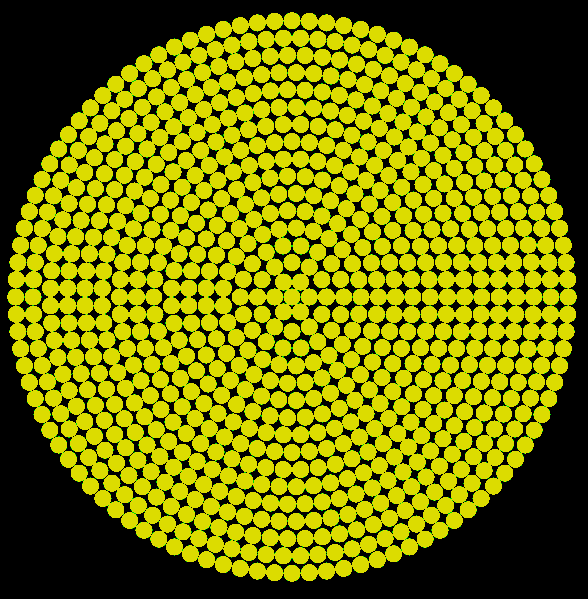
\includegraphics[scale=0.4]{6Simulations/64Tritium_IFIC_2/FiberDistribution_Tritium_IFIC_2_simulation.png}
\caption{Distribution of the scintillating fibers in the simualtion of Tritium-IFIC 2 prototype.\label{fig:FibersTritiumIFIC2Simulation}}
\end{figure}

The tritiated water source used consists of a tritiated water volume with a thickness of $5~\mu\meter$ around each scintillating fiber.

Scintillator fibers are located inside of a teflon vessel, which was simulated with the dimensions mentioned in section \ref{subsec:TritiumIFIC2}. Two PMMA windows with a thickness of $5~\mm$ were simulated and located in both fiber ends and a optical grease layer with a thickness of $0.5~\mm$ was included in each PMMA windows.

Finally, two PMTs, model R8520-460 from Hamamatsu company \cite{DataSheetPMTs}, were simulated in both ends. 

The optical properties used for the tritiated water, teflon vessel, PMMA windows and the optical grease, mentioned in section \ref{sec:Geant4Environment}, are included in this simulation. 

The simulation of TRITIUM-IFIC 2 is shown in Figure \ref{fig:TritiumIFIC2Simulation} in which can be appreciated the PMTs (black), the optical grease (blue), PMMA windows (white), tritiated water (green) and scintillating fibers (yellow). In this image, the Teflon container was not drawn to allow its interior to be seen and several volumes of tritiated water were also not included to allow several scintillation fibers to be seen.

\begin{figure}[h]
\centering
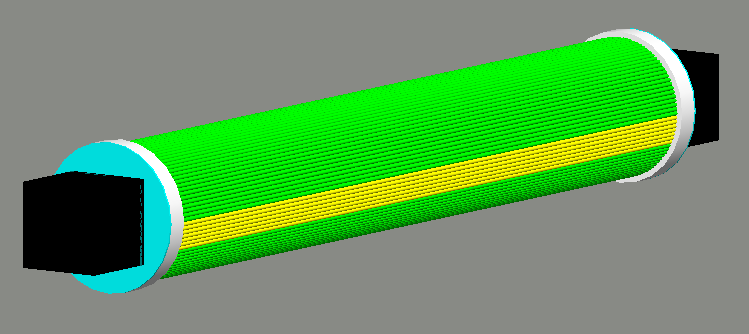
\includegraphics[scale=0.4]{6Simulations/64Tritium_IFIC_2/SimulationTritiumIFIC2.png}
\caption{Simualtion of Tritium-IFIC 2 prototype. PMTs (black), the optical grease (blue), PMMA windows (white), tritiated water (green) and scintillating fibers (yellow). \label{fig:TritiumIFIC2Simulation}}
\end{figure}

As can be seen in this figure, the used PMTs don't cover the entire active area formed by the scintillating fiber bundle. It's not a problem for the Tritium detector since its final version will not include this photosensors. The final version of Tritium-IFIC 2 prototype will use SiPM arrays and the PMTs model used in the Tritium-Aveiro 0 prototype are circular PMTs with which the full active area is covered.

The simulation of the Tritium-Aveiro 0 prototype is similar to this since the design of both detectors are quite similar. There are two main difference between both simulated prototypes:

\begin{enumerate}

\item{} The diameter of the fibers used, which is $1~\mm$ for Tritium-IFIC 2 prototype and $2~\mm$ for Tritium-Aveiro 0 prototype. As the internal volume of the teflon vessel is filled, this difference imply a difference number of the scintillating fibers used, causing a difference in the signal-background ratio.

\item{} The photosensors used since, although both are PMTs, the model of the used PMTs is different and it cause a different active area readout, affecting to the tritium detection efficiency. 

\end{enumerate}

The results obtained with the simulation of the TRITIUM-IFIC 2 prototype are shown in section \ref{subsec:ResultsSimulatedTRITIUMIFIC2}, where they are discussed.